%!TEX root = ../main.tex
%%%%%%%%%%%%%%%%%%%%%%%%%%%%%%%%%%
% Links: https://codereview.stackexchange.com/questions/252242/floyds-cycle-finding-algorithm
%
% Difficulty: Companies: 
%%%%%%%%%%%%%%%%%%%%%%%%%%%%%%%%%%

\chapter{Find the cycle in a Linked list}
\label{ch:cycle_in_list}
\section*{Introduction}
The problem described in this chapter is a classical one that has been reported to be asked in 
in countless coding interviews. The topic of this chapter is linked-lists: linear collections of elements whose order, unlike an array,
is not dictated by their ordering in memory. 
By being one of the most simple and common data structures you can expect them to be as important for your interview preparation.

The major difference that lists offer over conventional arrays is that elements in the list can be efficiently  (in constant time) 
removed and inserted without the need to reorganize and perform a complete restructuring of the whole data \footnote{For arrays, the cost of inserting or deleting an element is linear as you need to:
\begin{enumerate*}
	\item possibly enlarge the allocated space for the array
	\item copy all the elements (minus or plus the element you want to remove or insert) in the new memory space
\end{enumerate*}.
}. Because of this property linked lists are often used to implement more complex data structures 
where this insertion and deletion cost is crucial, for example associative arrays.
There are however quite a few drawbacks associated with them, for instance:
\begin{enumerate*}
	\item memory consumption (as for each node of the list you also pay a price as has to remember the next and/or previous nodes).
	\item they offer sequential access. Accessing a node costs linear time.
	\item cache unfriendly
\end{enumerate*}. This is the reason why  

A linked list is, at a high level of abstraction, a collection of so-called nodes or elements  each of them (except the last) containing
a pointer to the next one. 
Each node also carries payload data, which is the information you want ultimately to be stored.
The standard linked lists has two special nodes:
\begin{itemize}
	\item the head that is not pointed by other elements and is the first of the collection. 
	\item the tail, which is a node that has no next element, and is, not surprisingly, the last of the elements.
\end{itemize}

In some particular cases during the manipulation of the list you might end up with a broken or corrupted one  where the tail node does not exists anymore, meaning that
each of the elements in the list is pointing to some other nodes.
In this situation a loop forms and the list becomes what it known as a \textit{circular} list.
In this chapter we will investigate how we can find out whether:
\begin{enumerate*}
	\item a list is circular, and when it is,
	\item how to identify the first element of the loop.
\end{enumerate*}.

\section{Problem statement}
\begin{exercise}
Given a singly linked list (definition in Listing \ref{list:delete_duplicates_list:linked_list} at
page \pageref{list:delete_duplicates_list:linked_list}) determine whether the list contains a loop.
\begin{itemize}
		\item If it does, return the the node where the loop starts
		\item otherwise, return \lstinline[columns=fixed]{nullptr}
\end{itemize}

For the rest of the chapter we will use an array of integers to represents the nodes of the list and
a single integer to represent the node the last element of the list connects to, in order to create
a cycle or $-1$ if there is no cycle. For instance  the array $L=[1,2,3,4]$ and the integer $2$
represent the list shown in Figure \ref{fig:cycle_in_list:example1}.

\begin{example}
	\hfill \\
	Given the List $\{[1,2,3,4,5],2\}$, the function returns the address of the node $2$. See Figure
	\ref{fig:cycle_in_list:example1}.
\end{example}

\begin{example}
	\hfill \\
	Given the List $\{[1,2,3,4,5],-1\}$, the function returns \inline{nullptr}. See Figure
	\ref{fig:cycle_in_list:example2}.
\end{example}
\end{exercise}

\begin{figure}
	\centering
	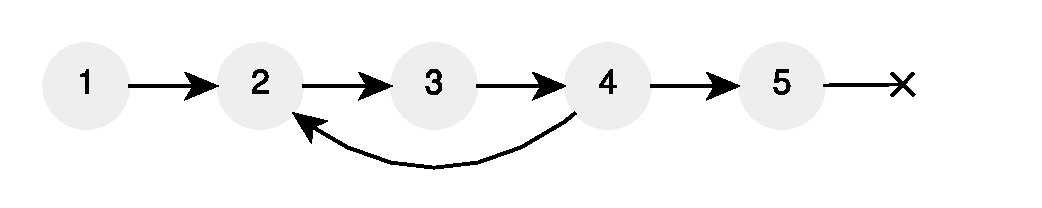
\includegraphics[scale=1.0]{sources/cycle_in_list/images/list_cycle}
	\caption{Example of linked list with a cycle.}
	\label{fig:cycle_in_list:example1}
\end{figure}
\begin{figure}
	\label{fig:cycle_in_list:example2}
	\centering
	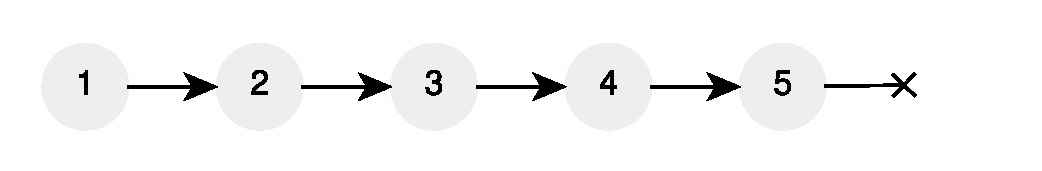
\includegraphics[scale=1.0]{sources/cycle_in_list/images/list_no_cycle}
	\caption{Example of linked list with no cycle.}
\end{figure}

%\section{Clarification Questions}
%
%\begin{QandA} \item \begin{answered} \textit{} \end{answered}
%
%\end{QandA}

\section{Discussion}
\label{cycle_in_list:sec:discussion}
Considering this is a very well-known problem we will not spent time on dwelling on naive
brute-force solution, and instead will only concentrate first on an optimal in time solution with
linear space, and then we will concentrate on improving it by lowering the space complexity to
constant. 

All solution implementation in this chapter uses the  Linked list definition shown in Listing \ref{list:cycle_in_list:node_definition};

\begin{minipage}{\linewidth}
	\lstinputlisting[language=c++, caption={Singly linked-list node definition.},label=list:cycle_in_list:node_definition]{sources/cycle_in_list/linked_list.h}
\end{minipage}

\subsection{Linear time and space solution}
\label{cycle_in_list:sec:bruteforce}
This problem has many similarities with the problem of finding a duplicate in a collection and can
therefore be solved using a similar approach. The idea is to visit the list and store in a hash-set
the  address of the node \textbf{already} visited. While visiting a new node, we first check if that
node was already visited, and if yes, it means that we can stop because we found the starting point
of a loop. If we reach the end of the list and we were not be able to find a duplicate, then it
means there is no loop and we can return \lstinline[columns=fixed]{nullptr}. A possible
implementation of this idea is shown in Listing \ref{list:cycle_in_list:linearspace}.

\lstinputlisting[language=c++, caption={Linear time and space solution to the problem of detecting a cycle in a linked list where an hashset is used to remember already visited nodes.},label=list:cycle_in_list:linearspace]{sources/cycle_in_list/cycle_in_list_solution1.cpp}



\subsection{Slow and fast pointer solution - Floyd’s algorithm }
\label{cycle_in_list:sec:slowfast}
This algorithm\cite{cit::wiki::floyd} uses the fact that, like clock's hands, things iterating on a
cycle at different speeds will eventually meet at some point in the future. Consider two runner $R_1$
and $R_2$ with velocities $V_1$ and $V_2=2V_1$ respectively ($R_2$ goes twice as fast then $R_1$),
starting their run from the same point in a circular stadium. They will meet again when the slower
runner reach the starting point for the second time. Why? By the time the slower one has completed
half circle the faster has completed a complete cycle and by the time the slower finishes his run,
arriving at the starting point again, the faster has completed a second entire cycle. We can use
this fact to detect a cycle in a linked list even if for the cycle detection problem things might be
a bit more complicated because the two runners might now start going in loop at the same time (the
list potentially has a first part the is not part of the loop as can be seen in Figure
\ref{fig:cycle_in_list:example1}). 


The rest of the section is a bit technical and you can skip to
the implementation shown in Listing \ref{list:cycle_in_list:constantspace} which can be self-explanatory considering that in the end the intuition behind the algorithm is quite easy. If you
are interested in the details of why it works, read along. 


Consider two iterators p,q with velocities $v_p=1$,$v_q=2$  respectively. Suppose the
\textbf{cycle}(not the entire list) has length $n$. We can have two scenarios depending on the index
$A$ of the starting node of the cycle:

\begin{enumerate}
\item the cycle starts at $A < n$.
\item or  starts at \(A \geq n\).
\end{enumerate}
For the case $(1)$ when the slower iterator reaches $A$ the faster is at location $2A$ (which might
mean that the faster iterator looped around the cycle already). How many iterations $k$ it will take
before they meet? And at which node?
The situation is described by the following congruences:
\begin{align}
  A + kv_p &\equiv 2A + k2v_p \Mod{n} \\
  2A + k2v_p &\equiv A + kv_p \;  \Mod{n} \\
  A + k2v_p &\equiv kv_p   \Mod{n} \\
  A +kv_p &\equiv 0   \Mod{n} \\
  A +k &\equiv 0  \Mod{n}
\end{align}
which has solution \(k = n-A\). This means that they will meet after \(k=n-A\) iterations of the
slower iterator, i.e. at \(A\) nodes before the beginning of the cycle and we can use this fact to
count \(A\) nodes from the beginning of the list so to find the starting point of the cycle. 

So, once the iterators meet \textbf{in the cycle}, we can move the fast iterator back to the
beginning of the list and iterate forward one node per step with both iterators until they match
again. When we move the fast iterator back at the head of the list, \textbf{both iterators are \(A\)
nodes away from the beginning of the cycle}. Because of this, when we move both of them by one, they
will eventually meet exactly at that node \(A\) i.e. the beginning of the cycle.

%%%------------

Let's consider now the case ($2$) i.e.  when \(A \geq n\). This means that by the time the slower
iterator reaches the beginning of the cycle the faster one has completed more that a cycle. What
will be the starting point for the faster one? We argue that once \(p\) reaches \(A\), \(q\) is at
node \(2A\) but since \(A > n\), this means that it will be at position \(A + (A \Mod{n})\). We can
now use similar argument to the previous case and write:

\begin{align}
  A + kv_p &\equiv A + (A \Mod{n}) + (k2v_p \Mod{n}) \\
  A + (A \Mod{n}) + k2v_p &\equiv A + kv_p\;\Mod{n} \\
  (A \Mod{n}) + kv_p \Mod{n} & \equiv 0\Mod{n} \\
  (A \Mod{n}) + k \Mod{n} &\equiv 0 \Mod{n} \: \: \text{  : because  } v_p=1 \\
\end{align}
which has solution \(k = n-(A \Mod{n})\). This means that the meeting point is \(A \Mod{n}\) nodes
before the beginning of the cycle. If we do the same operations as the previous case,(when \(A <
n\)), we obtain again, the same result. Iterators will meet at the beginning of the cycle. Why? Well
advancing \(q\) makes \(p\) cycle possibly several times ( remember that \(A \geq n\)  ) and it will
clearly stops at \( A+(n-A \Mod{n}) + A \Mod{n} = A +n \;(mod (n))= A\).
In other words the slower pointer is at first  at node number \(A+(n-A \Mod{n})\). We can write \( A
= bn + r\) where \(r = A \;\Mod{n}\). After \(A\) advancing steps it will be at location  \( A+(n-A
\;\Mod{n}) +bn +r (\Mod{n})\). Since \(bn \; \Mod{n}=0\) the result follows.

As an example consider a list with a cycle of length \(n=4\) starting at node number \(10\). The
first part of the algorithm tells us that the nodes will meet at node \(10 + 4 - 10 \: mod(4) =
12\). Moving the fast pointer back to the head of the list and iterating one node per time both
iterators will lead the slower point to node:


Figure \ref{fig:cycle_in_list:floyd} depicts how the algorithm
works on a list of $8$ nodes with a cycle of length $4$ starting at node number $4$. 
After $5$ steps the slow ($p$) and fast ($q$) iterators point to the same node i.e. node number $6$. 
After a new phase starts, with the slow pointer being moved to the head of the list and continues with both iterators moving forward by $1$
until they meet again. 
They will meet again at the beginning of the cycle. 

An implementation of the Floyd's algorithm is shown in Listing \ref{list:cycle_in_list:constantspace}.
\lstinputlisting[language=c++, caption={Floyd's algorithm, linear time, constant space solution to the problem of detecting a cycle in a linked list.},label=list:cycle_in_list:constantspace]{sources/cycle_in_list/cycle_in_list_solution2.cpp}


%\begin{figure}[htbp]
	%\label{fig:cycle_in_list:flow1} \centering
	%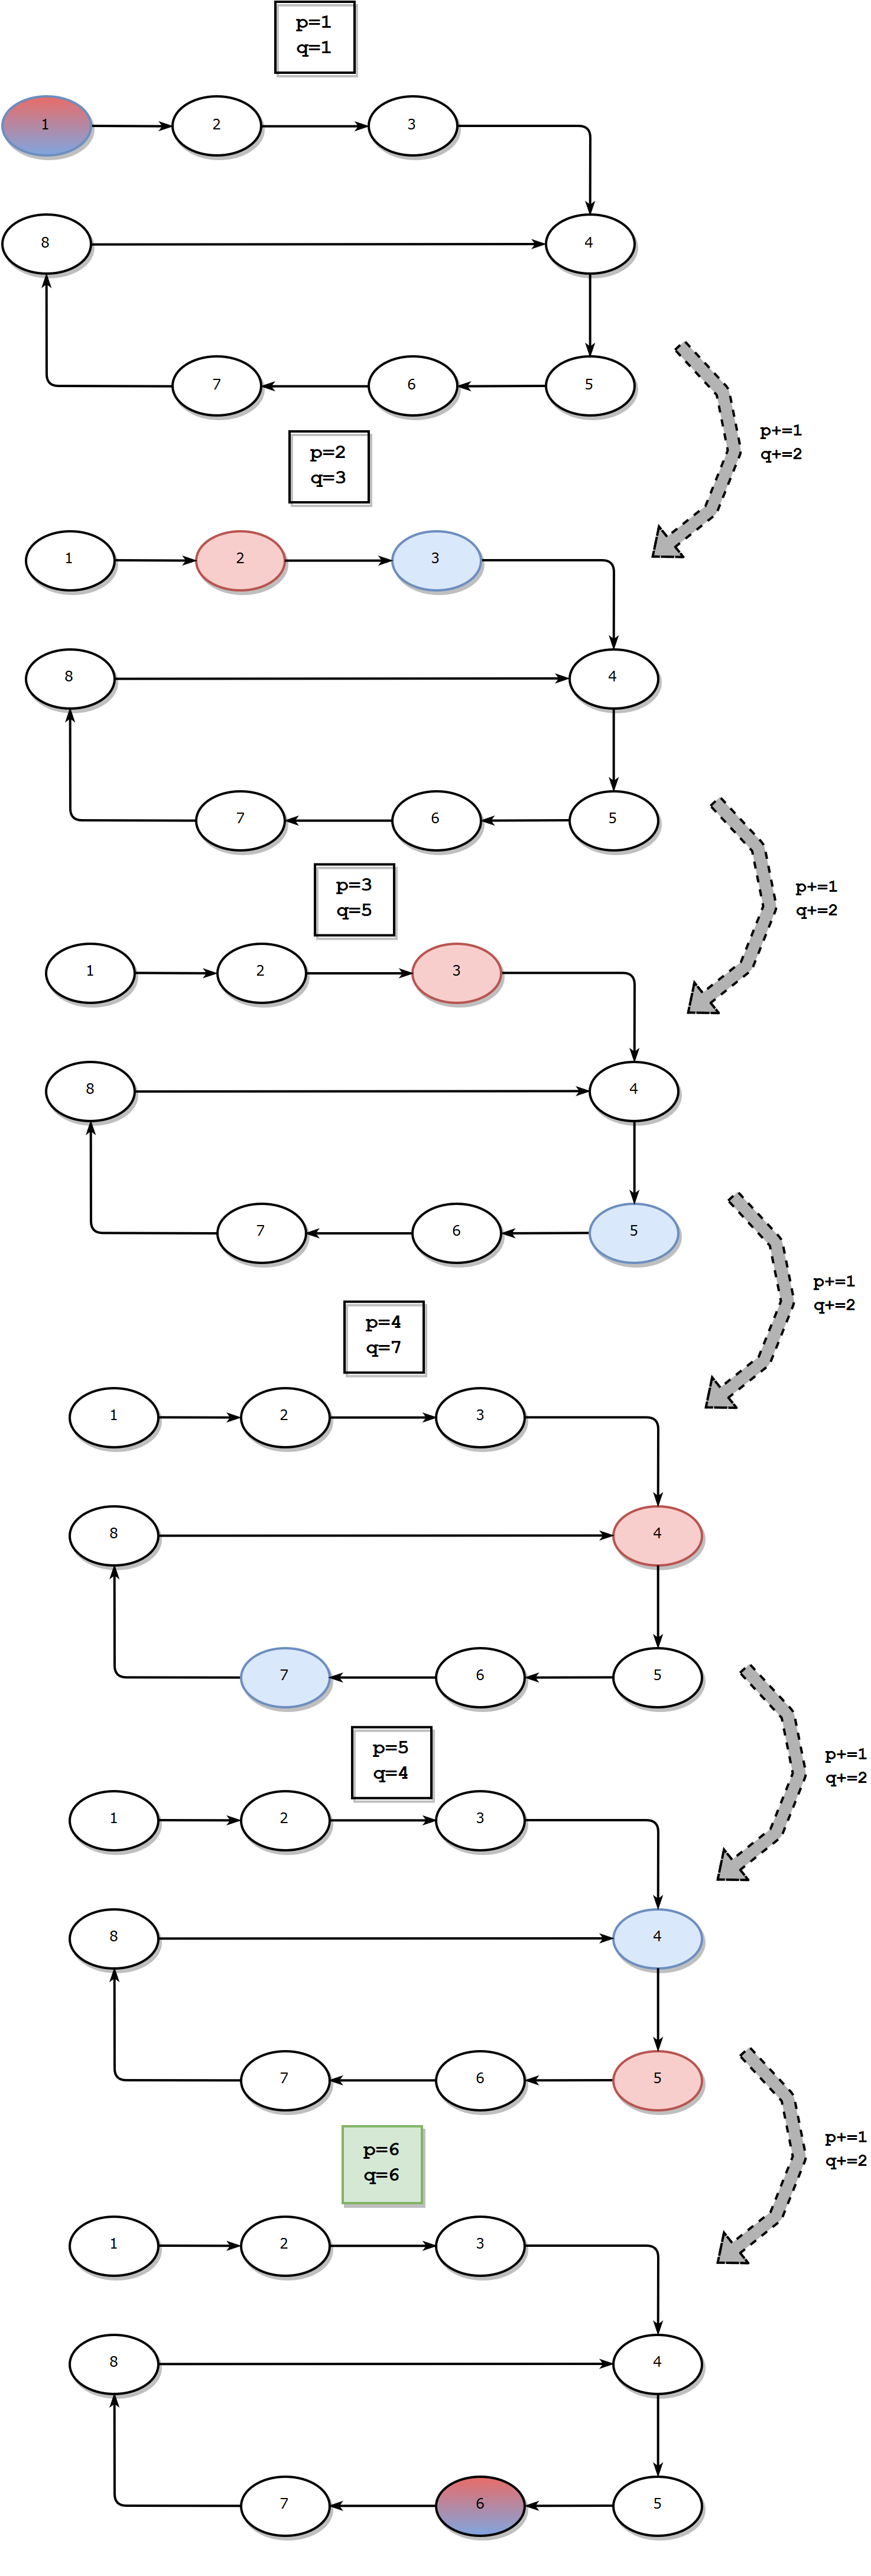
\includegraphics[scale=0.15]{sources/cycle_in_list/images/flow1} \caption{Execution of the
	%first phase of the Floyd's algorithm on a list of $8$ nodes with a cycle of length $4$ starting
	%at node $4$.}
%\end{figure}

%\begin{figure}[htbp]
	%\label{fig:cycle_in_list:flow2} \centering
	%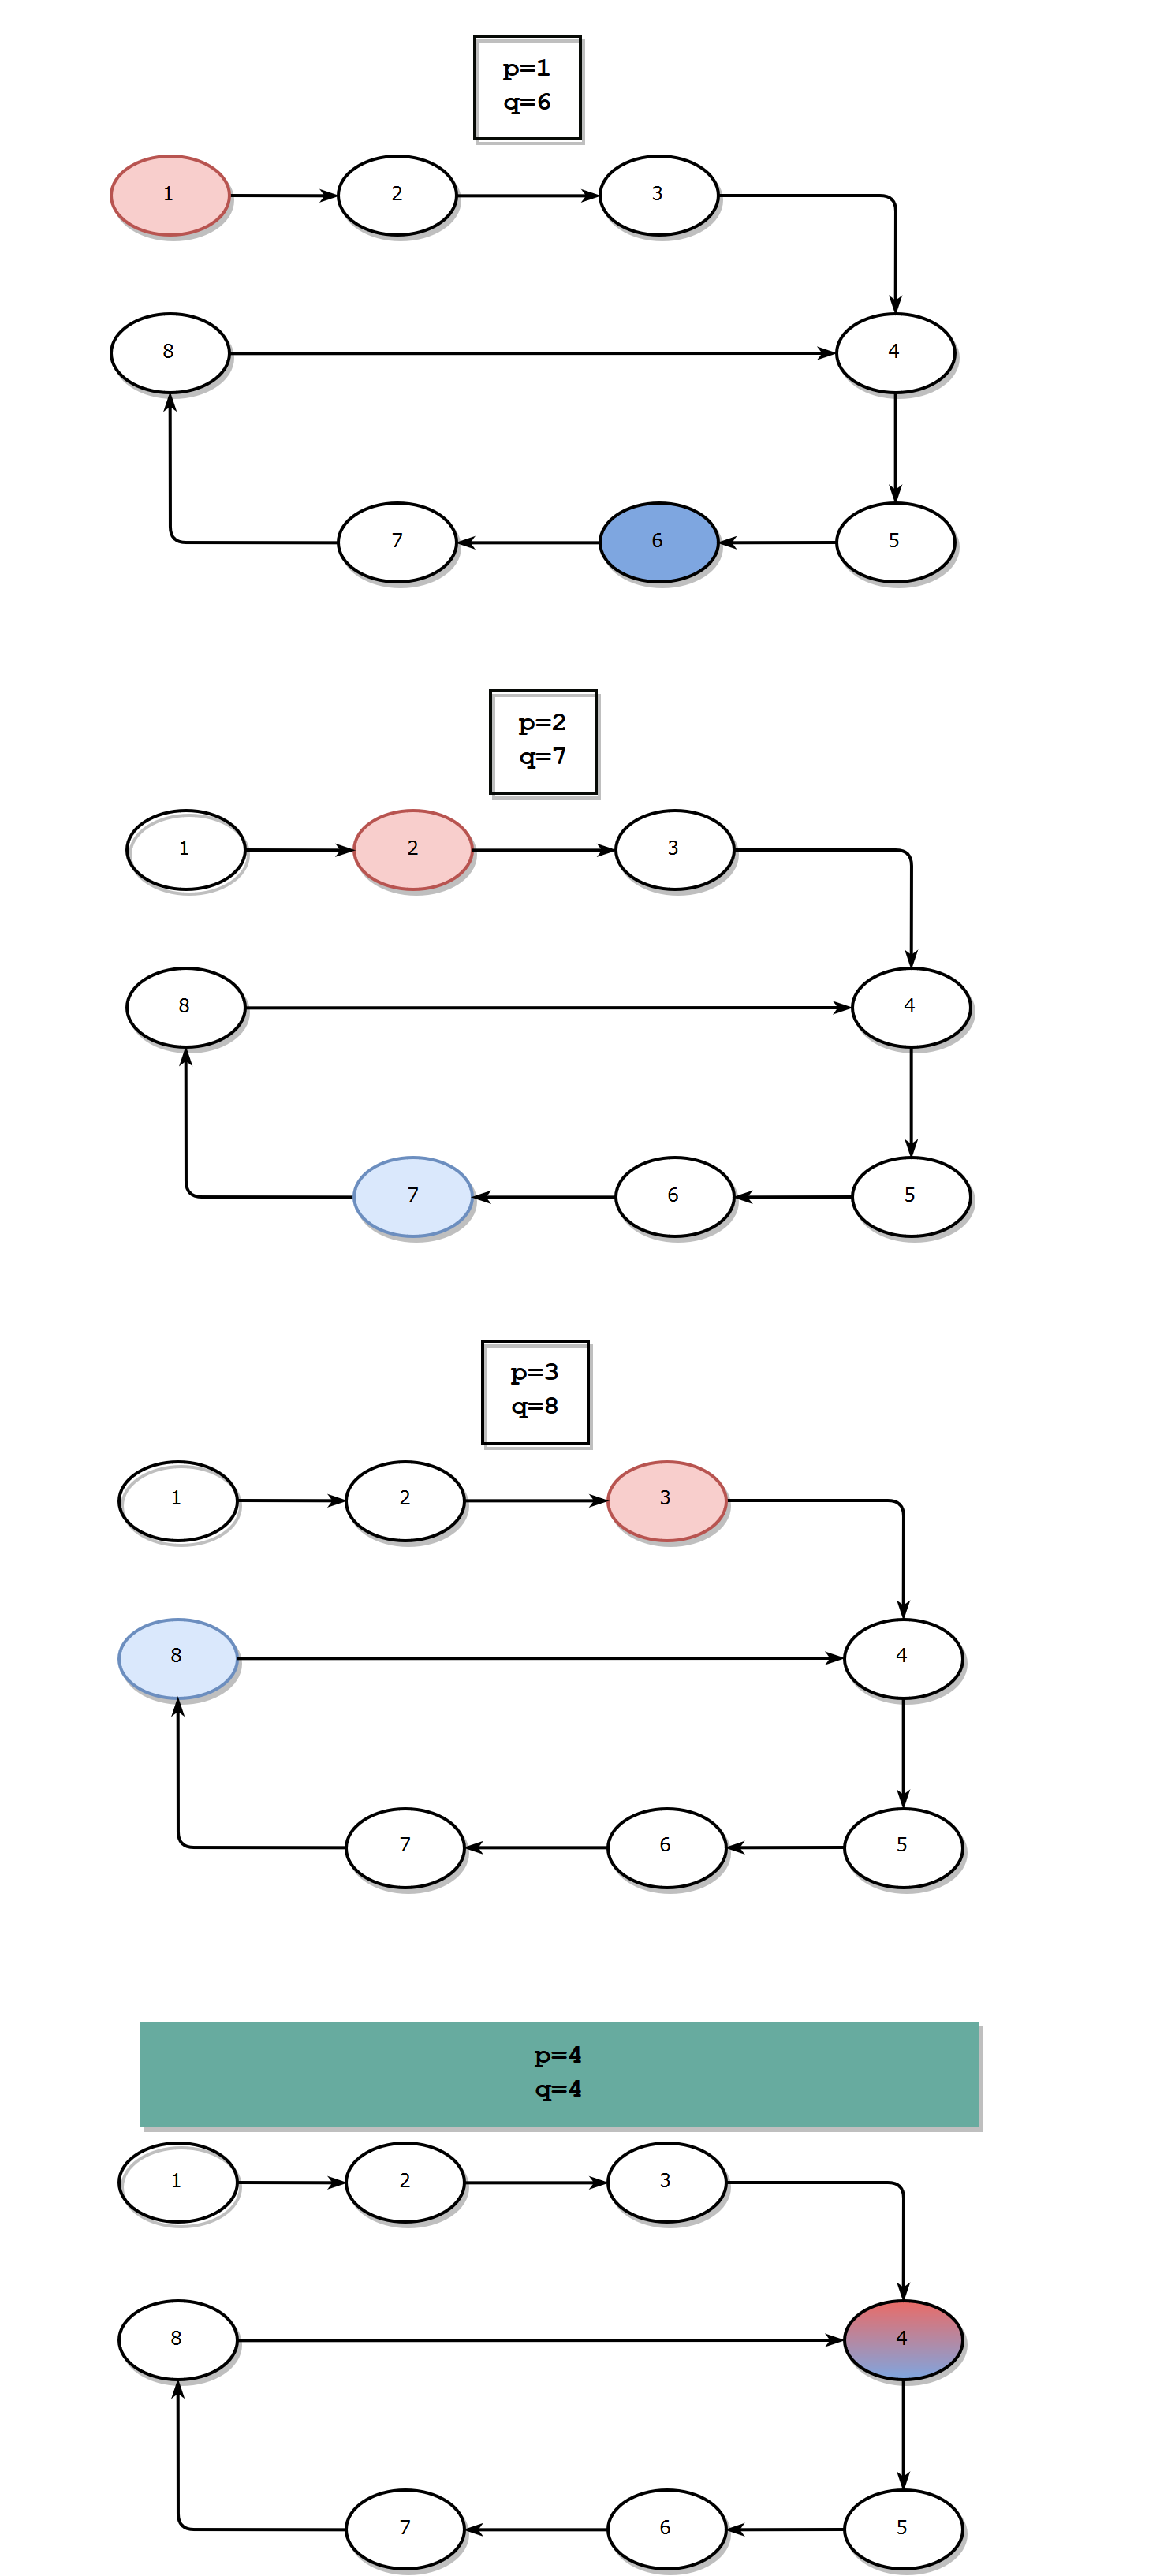
\includegraphics[scale=0.15]{sources/cycle_in_list/images/flow2} \caption{Execution of the
	%second phase of the Floyd's algorithm on a list of $8$ nodes with a cycle of length $4$
	%starting at node $4$.}
%\end{figure}




\begin{figure}
	\vspace*{-0.5in}
	\centering
	\begin{subfigure}[t]{0.36\textwidth}
		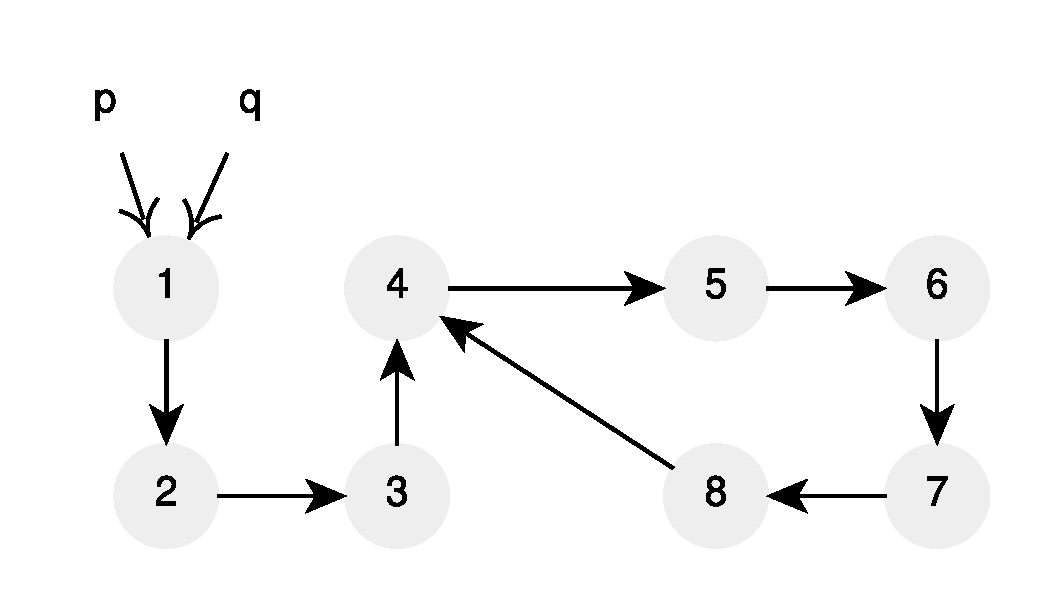
\includegraphics[width=1\linewidth]{sources/cycle_in_list/images/floyd1}
		\caption{At the beginning $p=q=1$. The slow and fast forward: $p=p+1$, $q=q+2$.}
		\label{fig:cycle_in_list:floyd1}
	 \end{subfigure}
	\hfill
	\begin{subfigure}[t]{0.36\textwidth}
		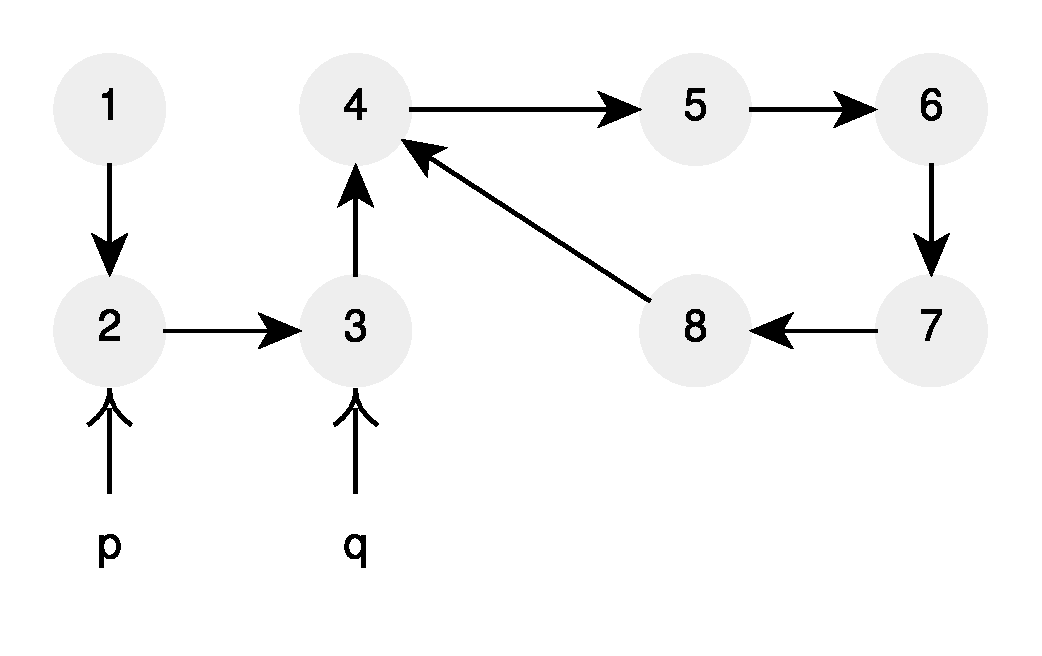
\includegraphics[width=1\linewidth]{sources/cycle_in_list/images/floyd2}
		\caption{$p \neq q$,  thus: $p=p+1$, $q=q+2$}
		\label{fig:cycle_in_list:floyd2}
	 \end{subfigure}
	 \hfill
	 \begin{subfigure}[l]{0.36\textwidth}
		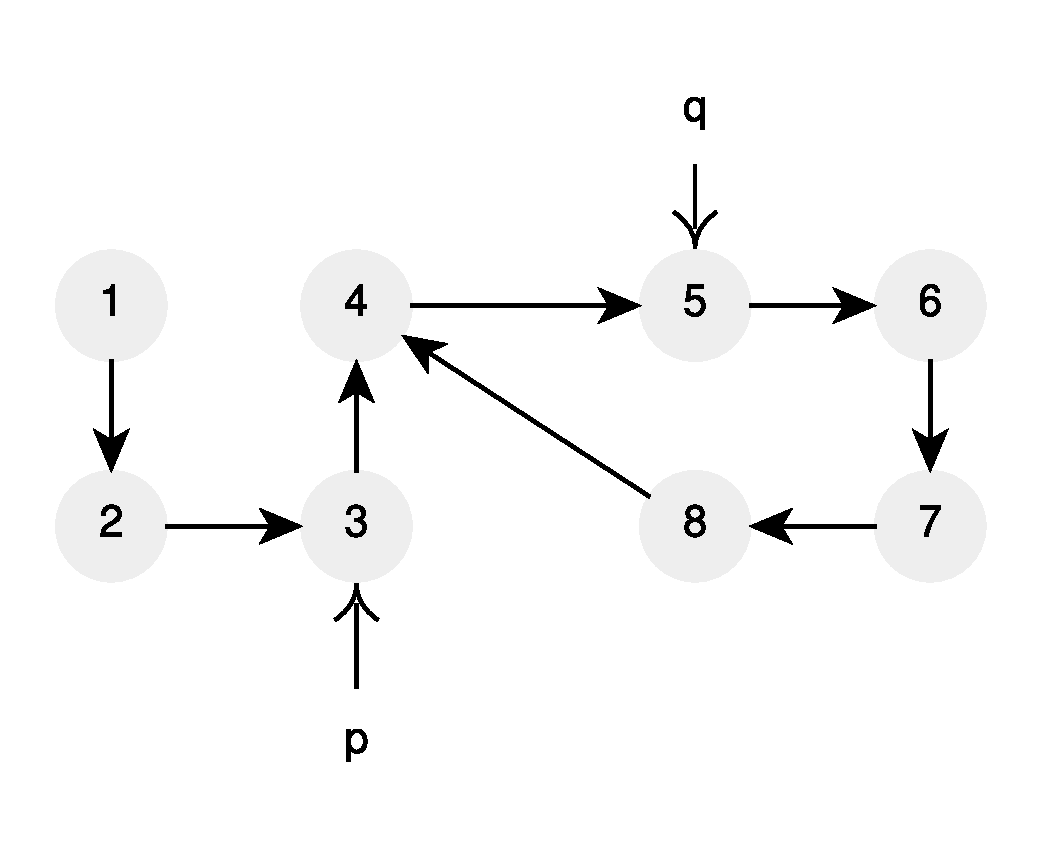
\includegraphics[width=1\linewidth]{sources/cycle_in_list/images/floyd3}
		\caption{$p \neq q$,  thus: $p=p+1$, $q=q+2$}
		\label{fig:cycle_in_list:floyd3}
	 \end{subfigure}
	 \hfill
	 \begin{subfigure}[l]{0.36\textwidth}
		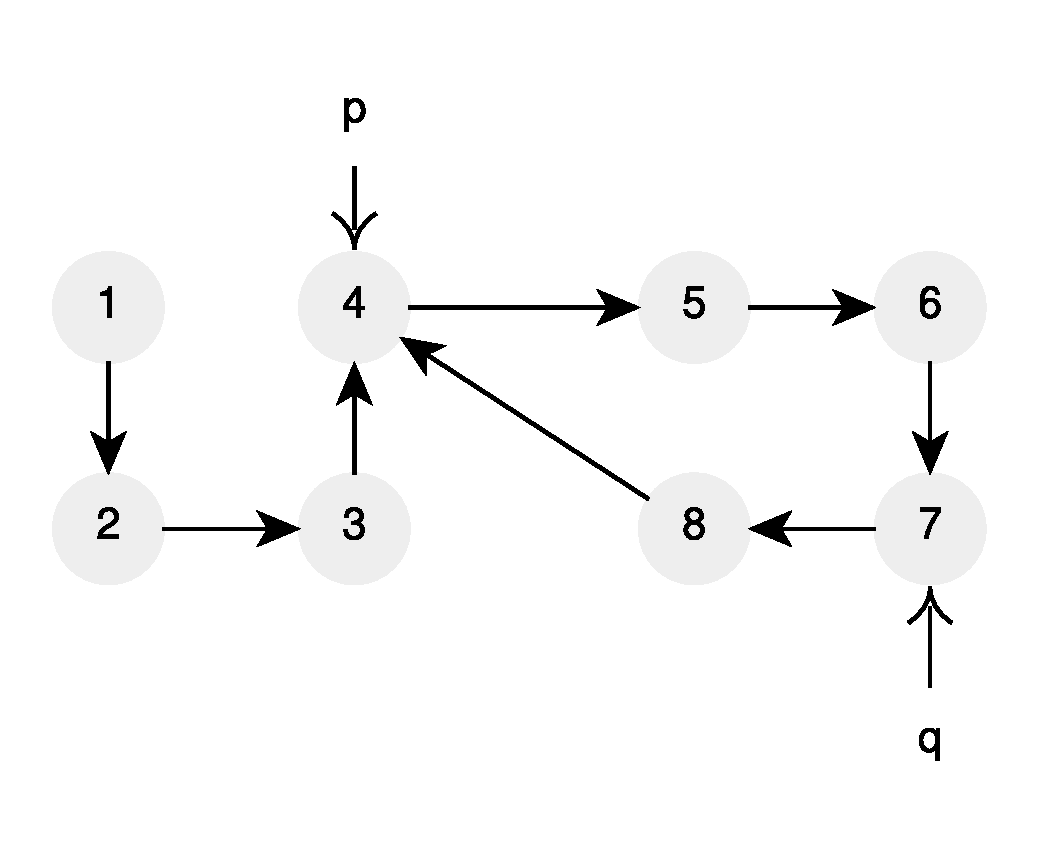
\includegraphics[width=1\linewidth]{sources/cycle_in_list/images/floyd4}
		\caption{$p \neq q$,  thus: $p=p+1$, $q=q+2$}
		\label{fig:cycle_in_list:floyd4}
	 \end{subfigure}
	 \hfill
	 \begin{subfigure}[l]{0.36\textwidth}
		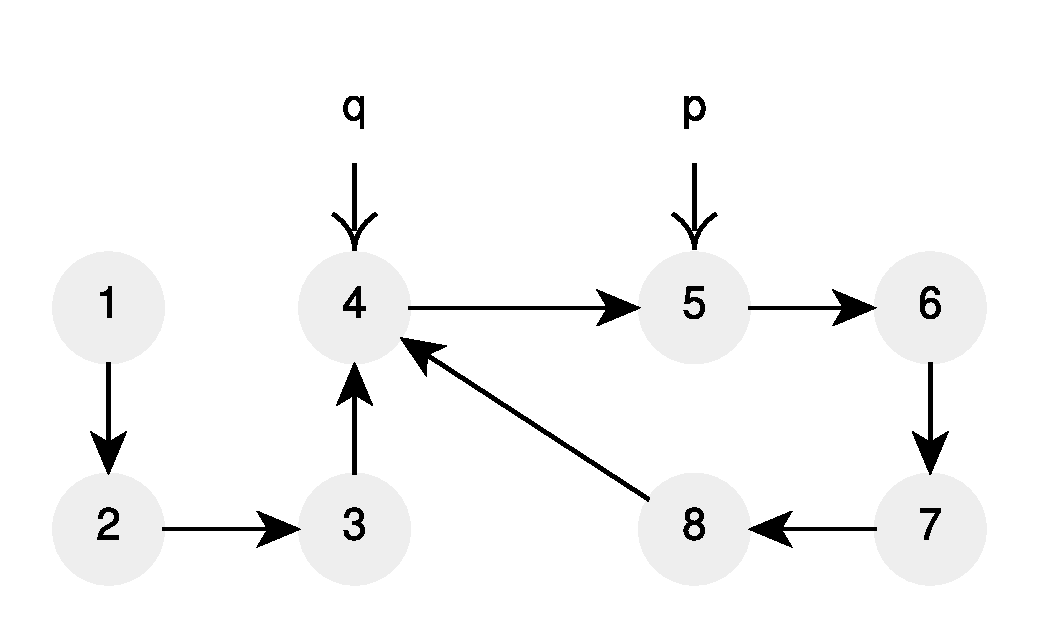
\includegraphics[width=1\linewidth]{sources/cycle_in_list/images/floyd5}
		\caption{$p \neq q$,  thus: $p=p+1$, $q=q+2$}
		\label{fig:cycle_in_list:floyd5}
	 \end{subfigure}
	 \hfill
	 \begin{subfigure}[l]{0.36\textwidth}
		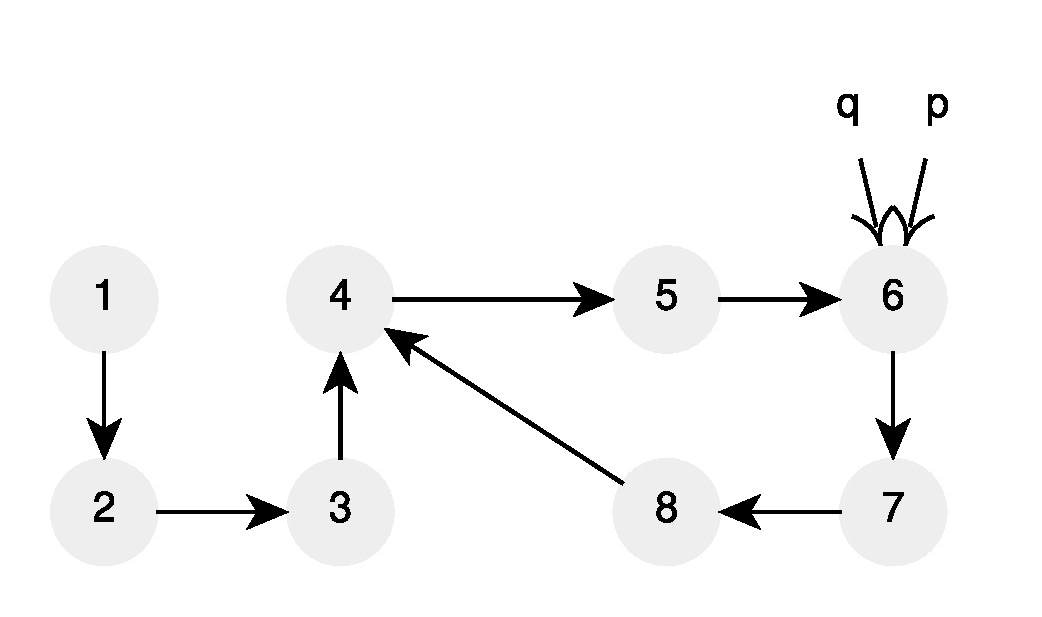
\includegraphics[width=1\linewidth]{sources/cycle_in_list/images/floyd6}
		\caption{$p = q$. The fast and slow movements stop.}
		\label{fig:cycle_in_list:floyd6}
	 \end{subfigure}
	 \hfill
	 \begin{subfigure}[l]{0.36\textwidth}
		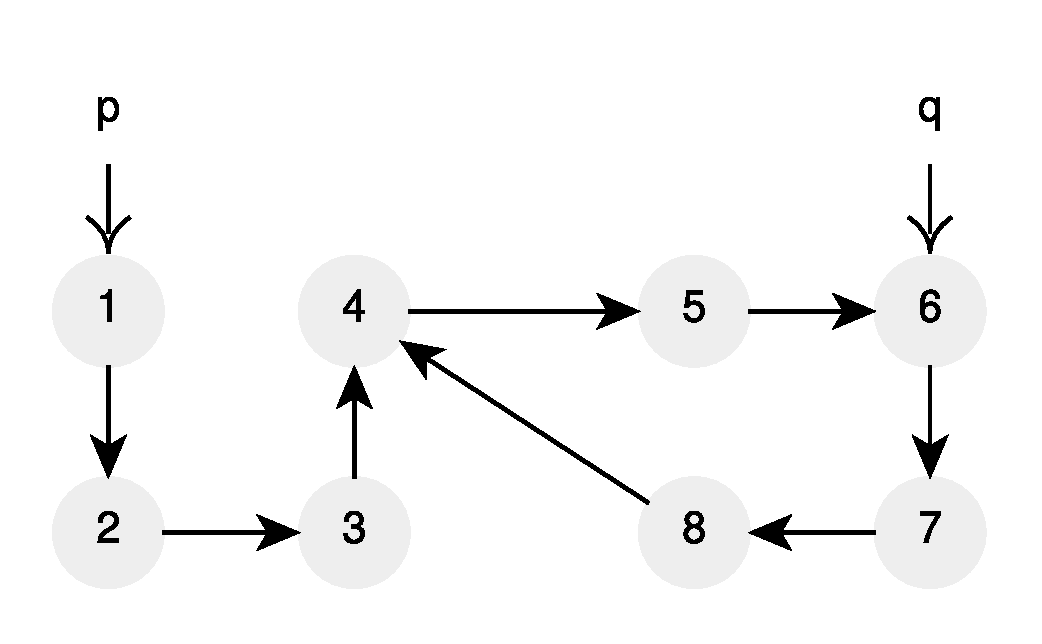
\includegraphics[width=1\linewidth]{sources/cycle_in_list/images/floyd7}
		\caption{$p$ is reset to the beginning of the list. $q$ is not moved.  
		From now on $p$ and $q$ are moved one step at the time.}
		\label{fig:cycle_in_list:floyd7}
	 \end{subfigure}
	 \hfill
	 \begin{subfigure}[l]{0.36\textwidth}
		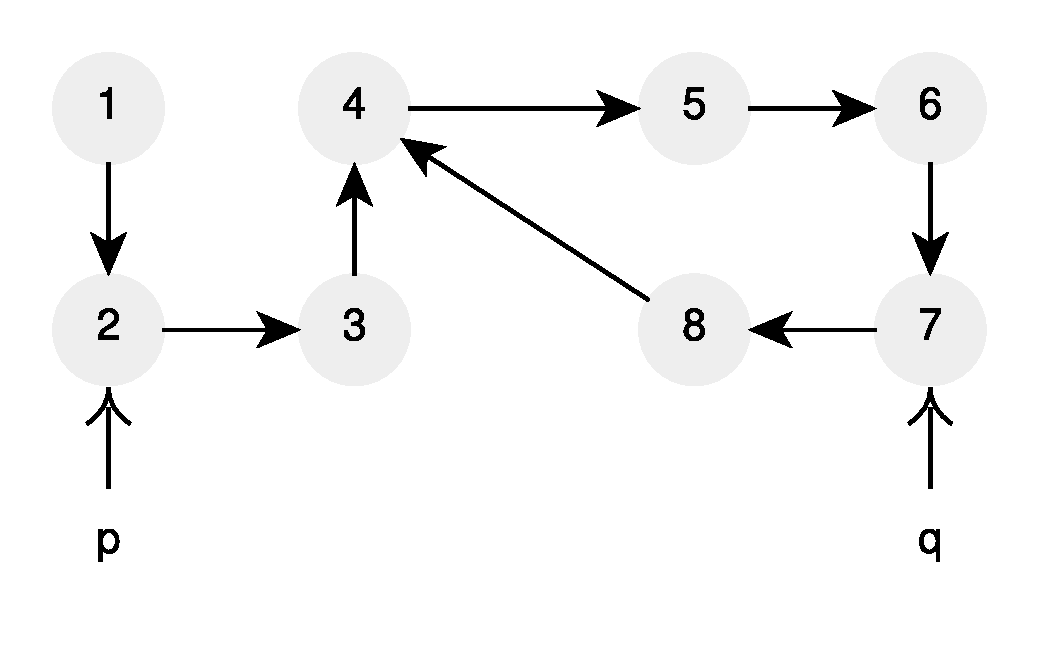
\includegraphics[width=1\linewidth]{sources/cycle_in_list/images/floyd8}
		\caption{$p \neq q$,  thus: $p=p+1$, $q=q+1$}
		\label{fig:cycle_in_list:floyd8}
	 \end{subfigure}
	 \hfill
	 \begin{subfigure}[l]{0.36\textwidth}
		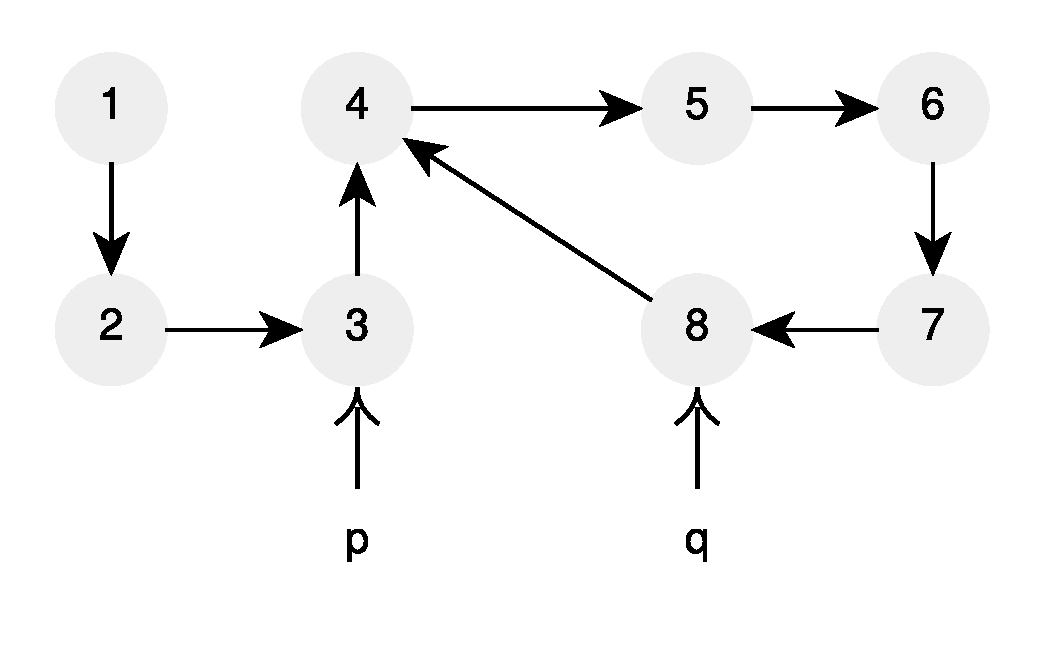
\includegraphics[width=1\linewidth]{sources/cycle_in_list/images/floyd9}
		\caption{$p \neq q$,  thus: $p=p+1$, $q=q+1$}
		\label{fig:cycle_in_list:floyd9}
	 \end{subfigure}
	 \hfill
	 \begin{subfigure}[l]{0.36\textwidth}
		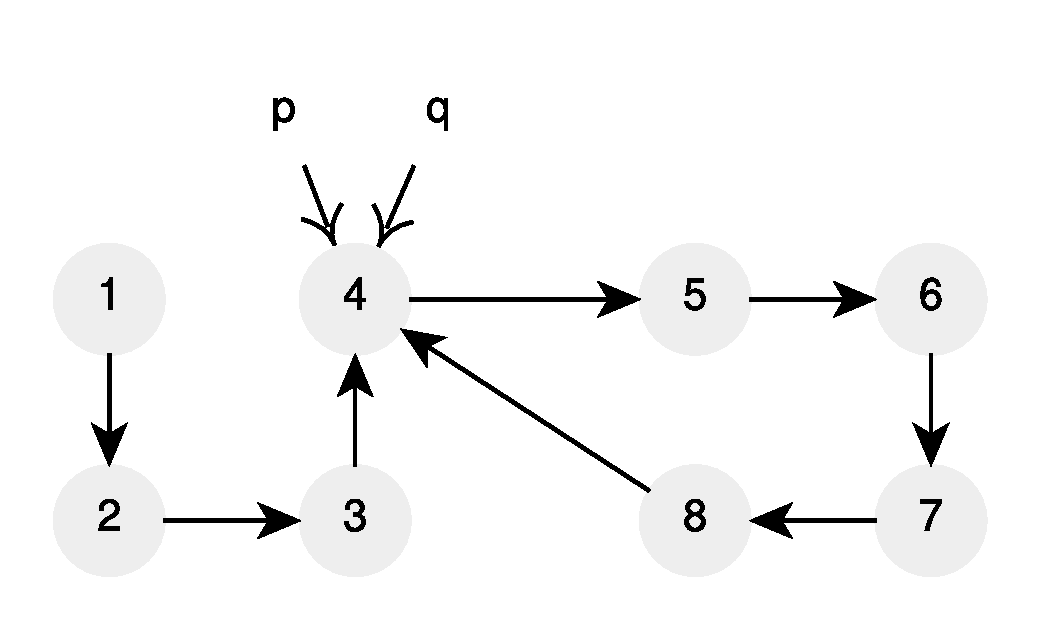
\includegraphics[width=1\linewidth]{sources/cycle_in_list/images/floyd10}
		\caption{$p = q$. The algorithm stops, and both $p$ and $q$ point to the beginning of the cycle.}
		\label{fig:cycle_in_list:floyd10}
	 \end{subfigure}
	 \caption[Execution of the Floyd’s algorithm]{Execution of the Floyd’s algorithm. The slow and
	  fast pointers are initialized to the head of the list (see Figure
	  \ref{fig:cycle_in_list:floyd1}) and immeditely moved forward at different speeds (Figure
	  \ref{fig:cycle_in_list:floyd2}). They continue to move forward at different speed until their
	  values mismatch (from Figure \ref{fig:cycle_in_list:floyd2} to
	  \ref{fig:cycle_in_list:floyd6}). At this point $p$ is moved back to the head of the list
	  (Figure \ref{fig:cycle_in_list:floyd7}). From now on the pointers are moved at the same speed
	  of $1$ and they continue to move forward until they match again (from Figure
	  \ref{fig:cycle_in_list:floyd8} to \ref{fig:cycle_in_list:floyd10}.). $p$ and $q$ now point to
	  the beginning of the cycle in the list.}
	  \label{fig:cycle_in_list:floyd}
\end{figure}
